\chapter{Datengrundlage und Vorverarbeitung}
\label{ch:datengrundlage}

In diesem Kapitel wird die Datengrundlage für die Entwicklung eines \ac{CNN}-basierten \ac{QR}-Code-Detektors beschrieben. Es werden die Eigenschaften des Datensatzes, die Vorgehensweise bei der Bildvorverarbeitung sowie die Erstellung von Trainings-, Validierungs- und Test-Splits erläutert. Ziel ist es, eine robuste Pipeline zu etablieren, die realistische Störeinflüsse auf der Windschutzscheibe berücksichtigt und eine effektive \ac{RoI}-Extraktion ermöglicht.

\section{Dateneigenschaften}
\label{sec:dateneigenschaften}

\subsection{Datenerhebung}
\label{sec:datenerhebung}
Zur Abbildung des Szenarios aus der Aufgabenstellung wurden die Bilddaten gezielt unter realistischen Bedingungen erhoben. Im Fokus standen dabei Störeinflüsse wie Verschmutzung, Spiegelungen, Nässe und Schaum sowie weitere Objekte hinter der Windschutzscheibe.

Der Datensatz basiert überwiegend auf eigenen Aufnahmen. Hierfür wurden selbst gedruckte \ac{QR}-Codes in unterschiedlichen Größen hinter der Windschutzscheibe platziert und anschließend aus verschiedenen Perspektiven aufgenommen. Insgesamt entstanden ca. 400 eigene Bilder verteilt auf zwei Fahrzeuge: Ein Fahrzeug wurde bewusst stark verschmutzt (u.\,a. Erde/Blätter, Kies im Hintergrund), das zweite Fahrzeug wurde in der Waschanlage bzw. mit Schaum und nasser Scheibe aufgenommen. Ergänzend wurden weitere Teil-Datensätze anderer Gruppen integriert, sodass insgesamt neun Teil-Datensätze zur Verfügung stehen.

Da die spätere Lesbarkeitsprüfung des \ac{QR}-Codes eine ausreichende Detailtreue erfordert, wurde bei der Datenerhebung bewusst auf hochauflösendes Bildmaterial (4K-Klasse) geachtet.

\begin{figure}[H]
    \centering
    \begin{minipage}[t]{0.49\linewidth}
        \centering
        % Pfad anpassen:
        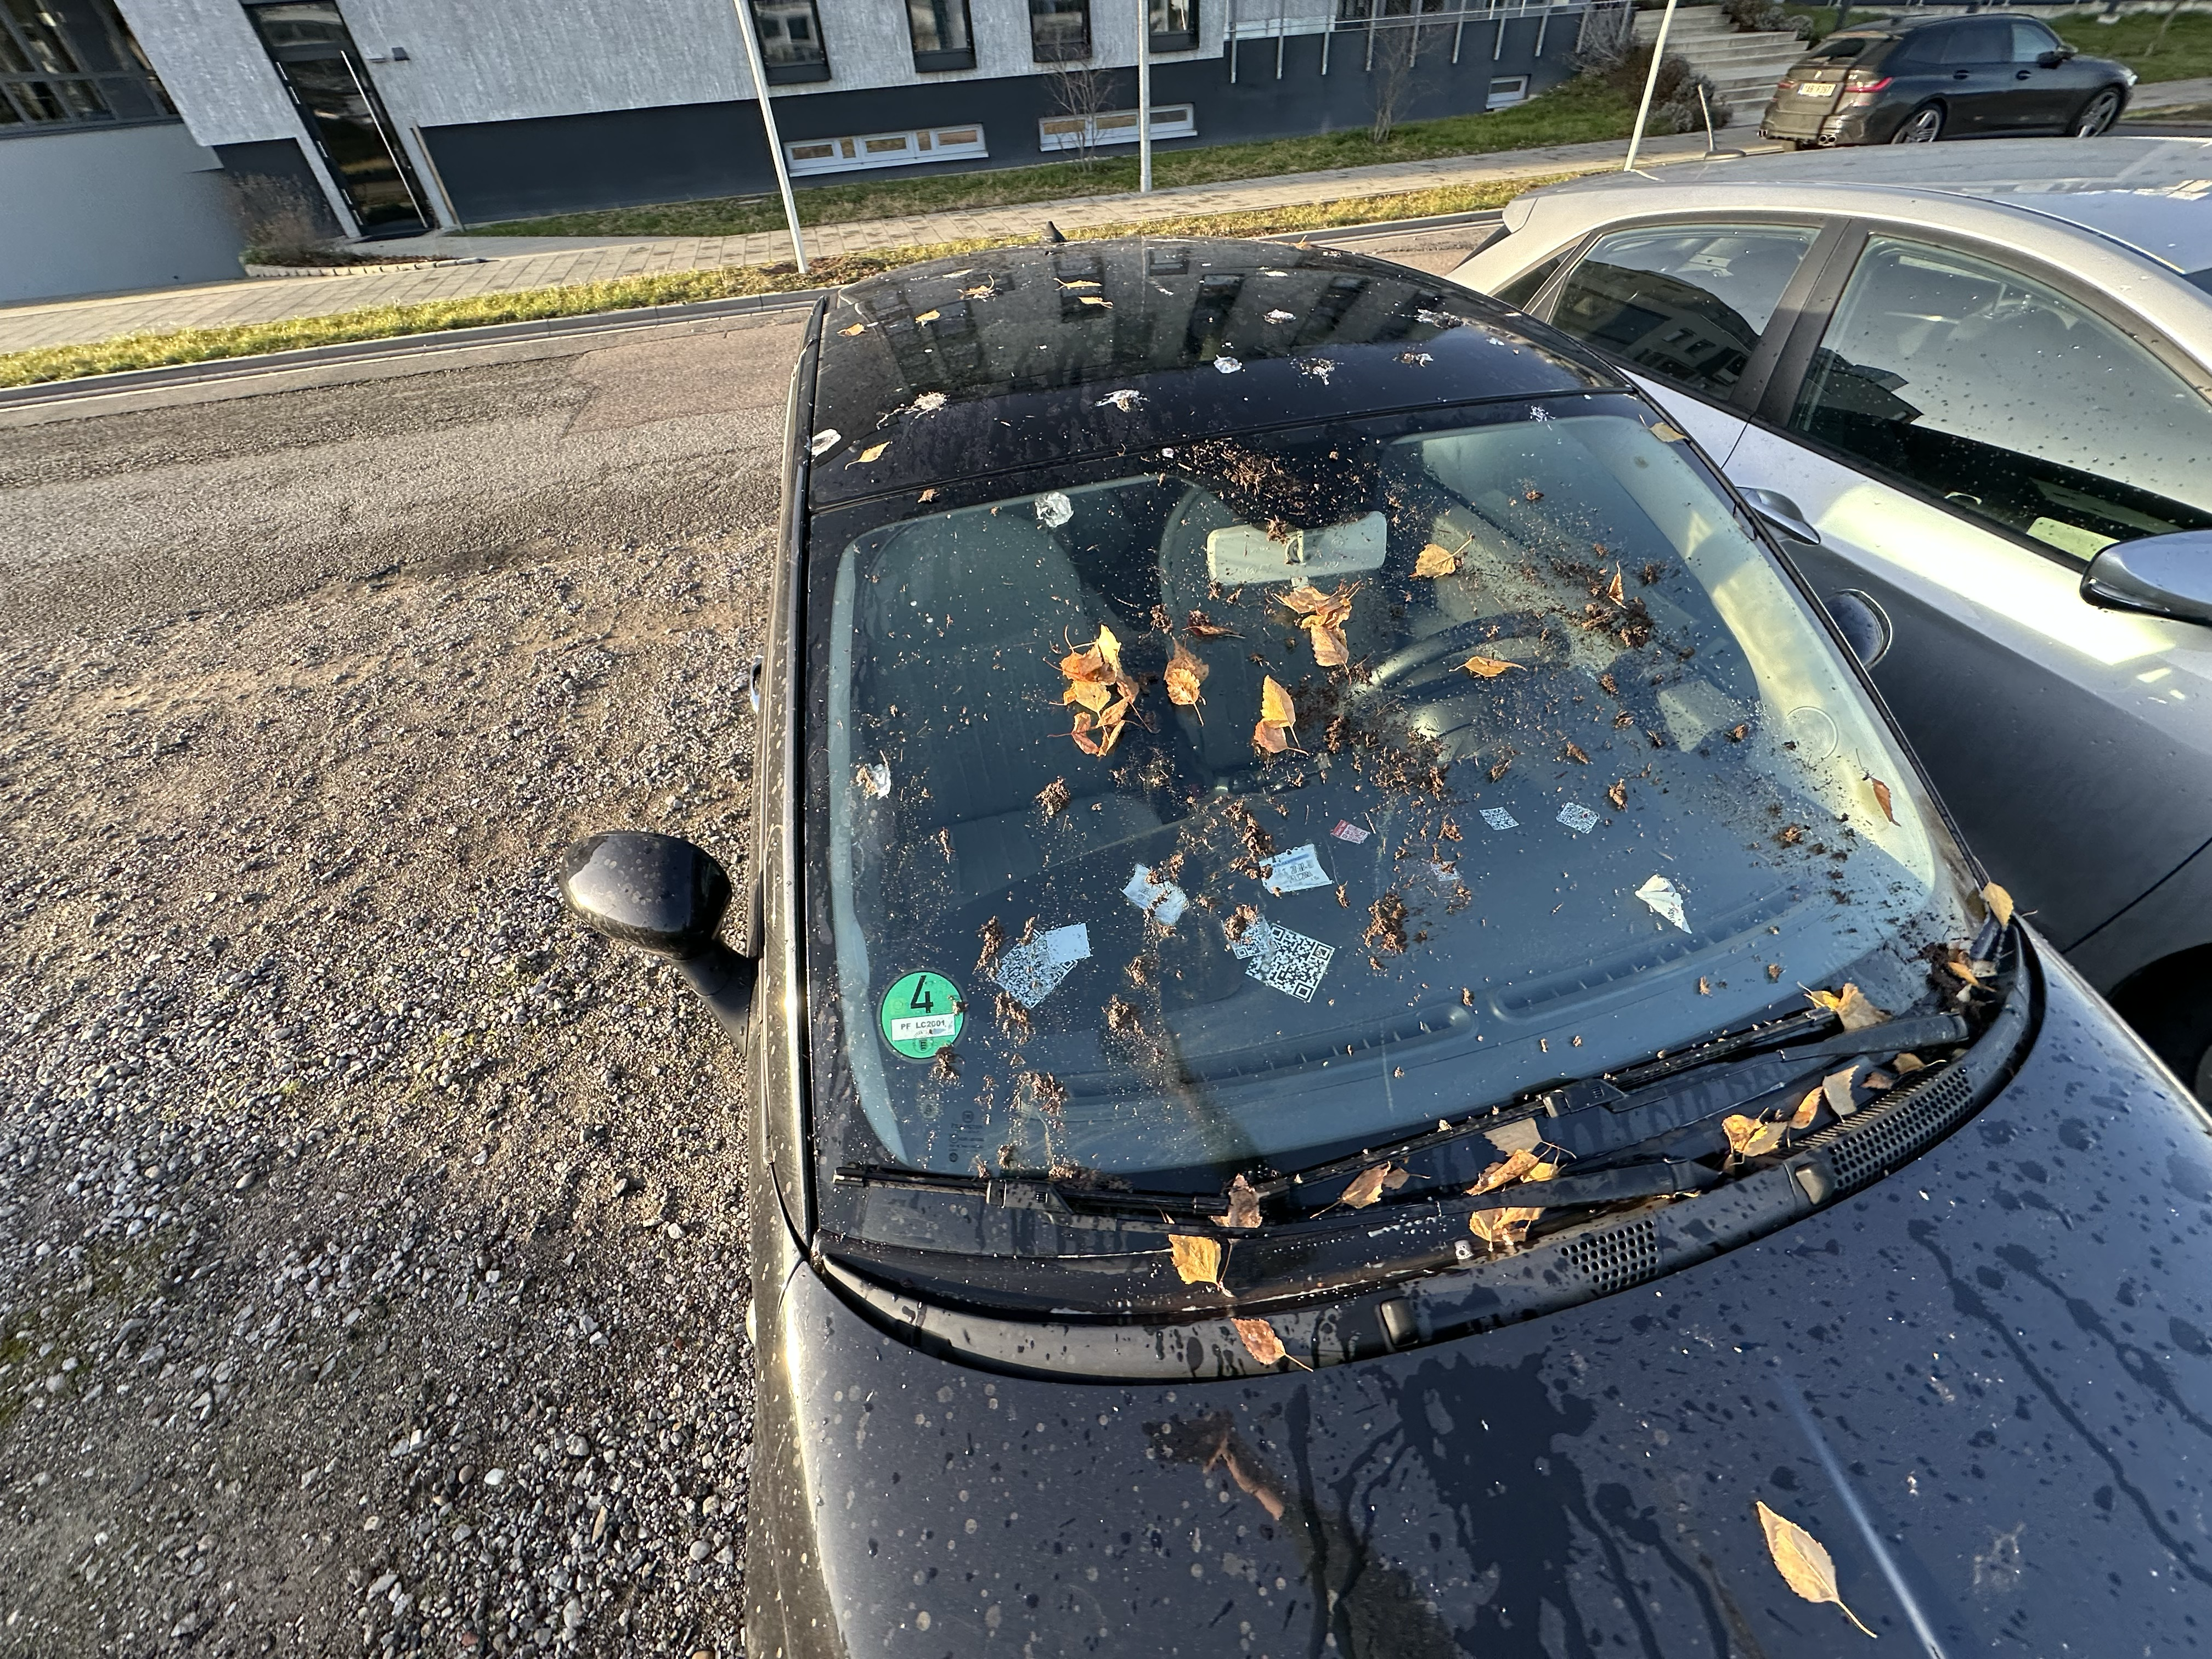
\includegraphics[width=\linewidth]{Figures/png/example_fiat_dirty.png}
        \caption*{(a) Fiat 500: stark verschmutzt, u.\,a. Kies/Reflexionen}
    \end{minipage}
    \hfill
    \begin{minipage}[t]{0.49\linewidth}
        \centering
        % Pfad anpassen:
        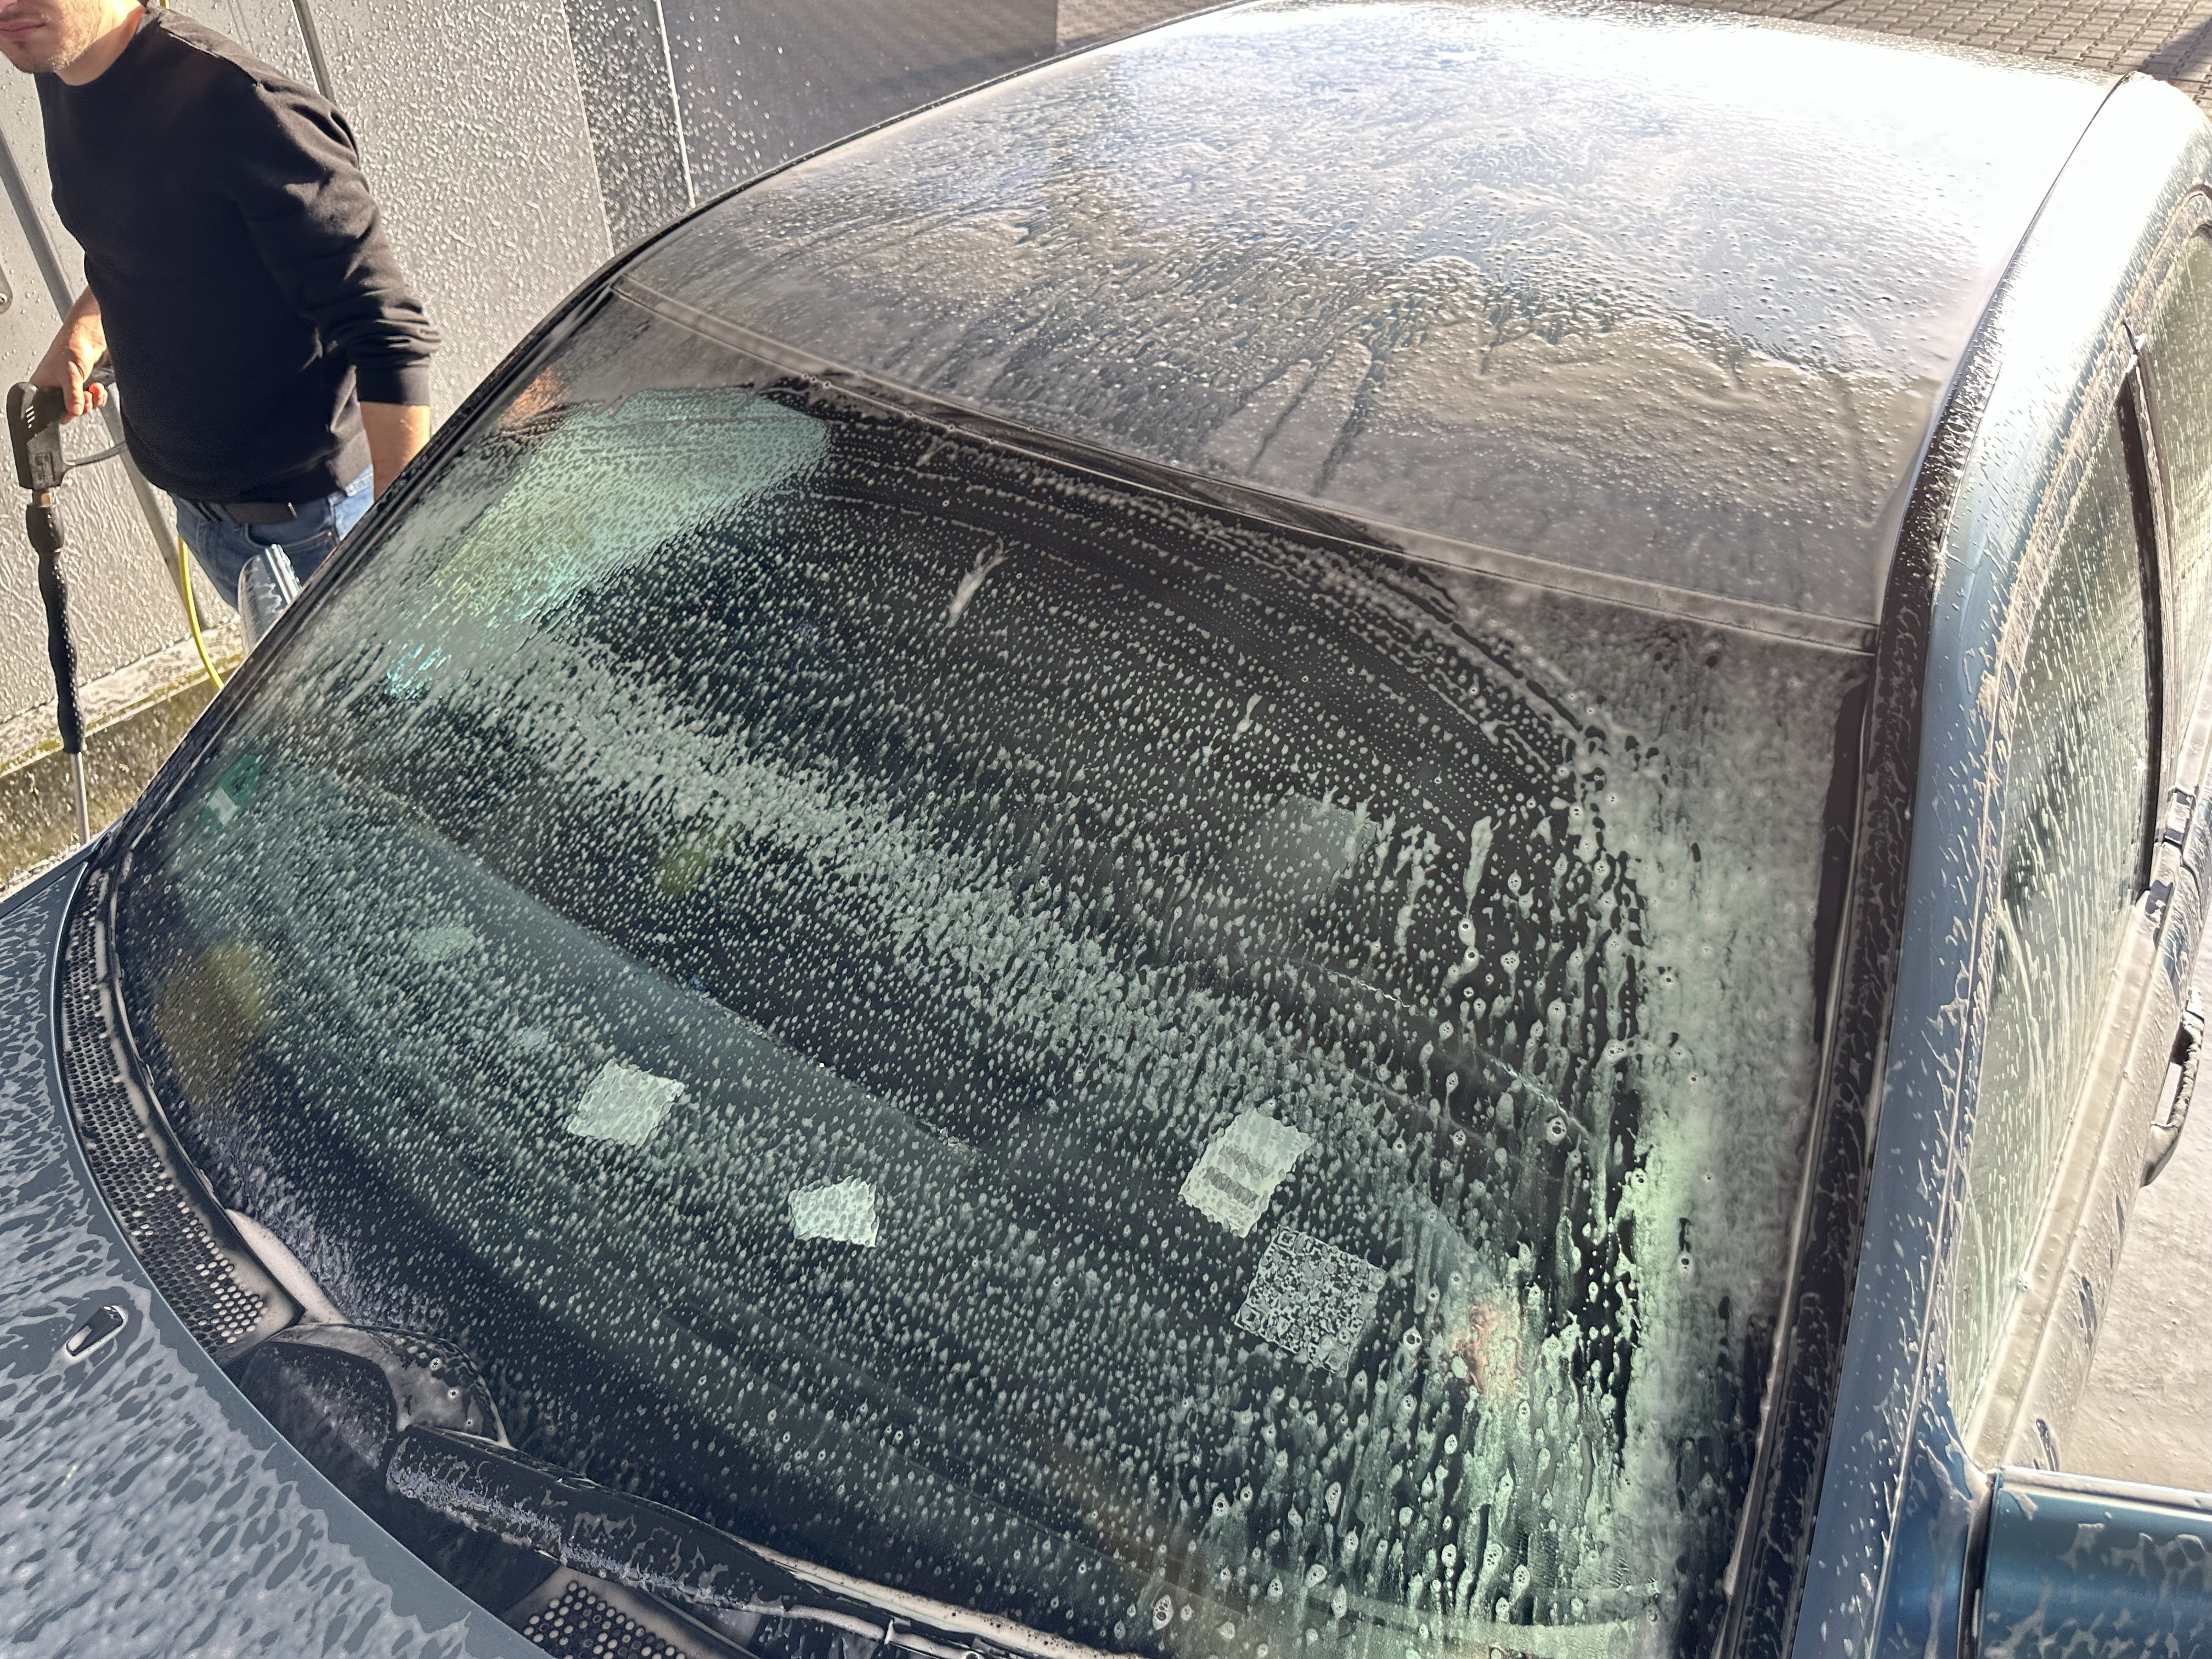
\includegraphics[width=\linewidth]{Figures/png/example_mercedes_foam.png}
        \caption*{(b) Mercedes W202: nasse/eingeschäumte Scheibe (Waschanlage)}
    \end{minipage}
    \caption{Beispielbilder aus den eigenen Aufnahmen: \ac{QR}-Codes hinter der Windschutzscheibe unter erschwerten Bedingungen.}
    \label{fig:dataset_examples}
\end{figure}

\subsection{Patch-Datensatz und Klassenverteilung}
\label{sec:patch_dataset}
Für das Training des \ac{CNN} wurde aus den hochauflösenden Bildern ein Patch-Datensatz aufgebaut. Hintergrund ist, dass der \ac{QR}-Code im Gesamtbild häufig nur einen kleinen Anteil einnimmt. Eine Patch-basierte Verarbeitung erlaubt es, relevante Bildbereiche in ausreichender Auflösung zu betrachten und dem \ac{CNN} eine konstante Eingabegröße bereitzustellen.

\begin{listNorm}
    \item \textbf{Patchgröße:} $265\,\times\,265$\,Pixel (konstante \ac{CNN}-Eingabe).
    \item \textbf{Manuelles Labeling:} ca. 26\,000 extrahierte Patches wurden manuell in \emph{\ac{QR}-Code} vs.~\emph{No \ac{QR}-Code} klassifiziert.
    \item \textbf{Augmentierung:} Rotation und horizontales Flippen der positiven \emph{\ac{QR}-Code}-Patches, um die positive Klasse zu erweitern und die Robustheit gegenüber Orientierungsvariationen zu erhöhen.
    \item \textbf{Klassenunwucht:} \emph{No \ac{QR}-Code} ist deutlich häufiger (insgesamt 49\,602 Patches nach Augmentierung) als \emph{\ac{QR}-Code}.
    \item \textbf{Positive Klasse:} rund 1\,500 \emph{\ac{QR}-Code}-Patches; nach Spiegelung ergeben sich 3\,066 \emph{\ac{QR}-Code}-Patches.
    \item \textbf{Balancierung:} Für das Training wird die negative Klasse pro Split zufällig auf die Größe der positiven Klasse heruntergesampelt (50/50).
\end{listNorm}

Die Aufteilung in Trainings-, Validierungs- und Testdaten erfolgt nicht durch Kopieren in neue Ordner, sondern wird als JSON-Datei gespeichert. Dabei werden Patches nach Quellbild gruppiert, um Datenleckage zu vermeiden (ein Quellbild erscheint nicht in mehreren Splits).

\newpage
\section{Bildvorverarbeitung}
\label{sec:bildvorverarbeitung}

\subsection{Motivation: Regionen statt Full-Image-Klassifikation}
\label{sec:roi_motivation}
Im Rahmen der Vorlesung wurde das Prinzip von Two-Stage-Detektoren vorgestellt, bei denen zunächst Kandidatenregionen (\emph{\ac{RoI}-Proposals}) bestimmt und anschließend klassifiziert werden. Dieser Gedanke wurde in diesem Projekt bewusst aufgegriffen, um erstmals eine Pipeline zu realisieren, die nicht nur das Gesamtbild klassifiziert, sondern gezielt Regionen extrahiert und einem \ac{CNN} zuführt. \cite{friedrich2025_cv,girshick2015_fast_rcnn}

Für das vorliegende Szenario ist dieser Ansatz insbesondere deshalb sinnvoll, weil \ac{QR}-Codes im Bild oft klein sind und bei starkem Downscaling des Gesamtbilds an Struktur verlieren. Durch die Patch-Erzeugung können relevante Bildbereiche in höherer Auflösung betrachtet werden und Störeinflüsse (Reflexionen, Schmutz, weitere Objekte) in Form negativer Beispiele explizit in den Trainingsprozess einfließen.

\subsection{ROI-Scoring: Heuristische Kandidatensuche}
\label{sec:roi_scoring}
Zur automatischen Erzeugung plausibler Kandidatenbereiche wird zunächst eine Score-Map berechnet, die pro Pixel eine \ac{QR}-ähnliche Strukturstärke repräsentiert. Die Score-Map kombiniert mehrere klassische Bildmerkmale, die für gedruckte \ac{QR}-Codes typisch sind:

\begin{listNorm}
    \item \textbf{Kanten (Canny):} \ac{QR}-Codes besitzen viele harte Schwarz/Weiß-Übergänge. Eine Kantenkarte liefert daher ein robustes Signal für strukturierte, kontrastreiche Bereiche.
    \item \textbf{Ecken (Harris):} Finder-Pattern und Modulraster erzeugen viele stabile Eckpunkte. Harris-Ecken sind daher ein geeignetes Indiz für \ac{QR}-ähnliche Regionen.
    \item \textbf{Gradientenstärke (Sobel-Magnitude):} Ergänzt Kanten/Ecken um ein kontinuierliches Kontrastmaß und stabilisiert die Bewertung bei wechselnden Schwellenwerten.
    \item \textbf{Anisotropie (Strukturtensor-basiert):} \ac{QR}-Codes enthalten regelmäßig ausgerichtete Kantenstrukturen. Ein Anisotropie-Maß hilft, solche Muster gegenüber flächigem Rauschen hervorzuheben.
\end{listNorm}

Die Merkmale werden gewichtet aufsummiert und anschließend normalisiert. In frühen Tests zeigte sich, dass Hintergrundobjekte mit starken Kanten/Ecken (z.\,B. Schlüssel oder Innenraumdetails) die Score-Map dominieren können. Die Gewichtung und Schwellwerte sind daher entscheidend, um die Spezifität für \ac{QR}-Codes zu erhöhen.
\newpage
\subsection{Multi-Scale Window Search und Redundanzreduktion}
\label{sec:roi_search}
Aus der Score-Map werden Kandidatenfenster über mehrere Skalen bestimmt:
\begin{listNorm}
    \item \textbf{Multi-Scale:} Abdeckung unterschiedlicher \ac{QR}-Code-Größen (Abstand/Zoom) durch mehrere Fenstergrößen.
    \item \textbf{Coarse-to-Fine:} Zunächst grobe Abtastung (großer Stride), anschließend lokale Verfeinerung um die besten Kandidaten (kleiner Stride).
    \item \textbf{Filterung über \ac{IoU}:} Stark überlappende Fenster werden unterdrückt, um redundante Patches zu vermeiden (Non-Maximum Suppression).
\end{listNorm}

Anschließend werden um die besten Kandidatenzentren quadratische Patches extrahiert und gespeichert. Optional werden zusätzlich gedrehte Varianten erzeugt, um geneigte Zettel und schräg platzierte \ac{QR}-Codes im Training abzudecken.

\subsection{Interaktives Parameter-Tuning (ROI-Tuner GUI)}
\label{sec:roi_gui}
Zur Parametrisierung der Score-Map und der Window-Suche wurde ein interaktives \ac{GUI} entwickelt. Dieses ermöglicht es, Gewichte und Schwellwerte live zu verändern und direkt zu beobachten, wie sich die Kandidatenfenster im Bild verhalten. Abbildung~\ref{fig:roi_tuner_gui} zeigt beispielhaft die Heatmap (links) sowie die Parametrierung über Regler (rechts). Die finalen Parameter werden als JSON-Konfiguration gespeichert und für die Batch-Extraktion verwendet.

\begin{figure}[H]
    \centering
    % Pfad anpassen:
    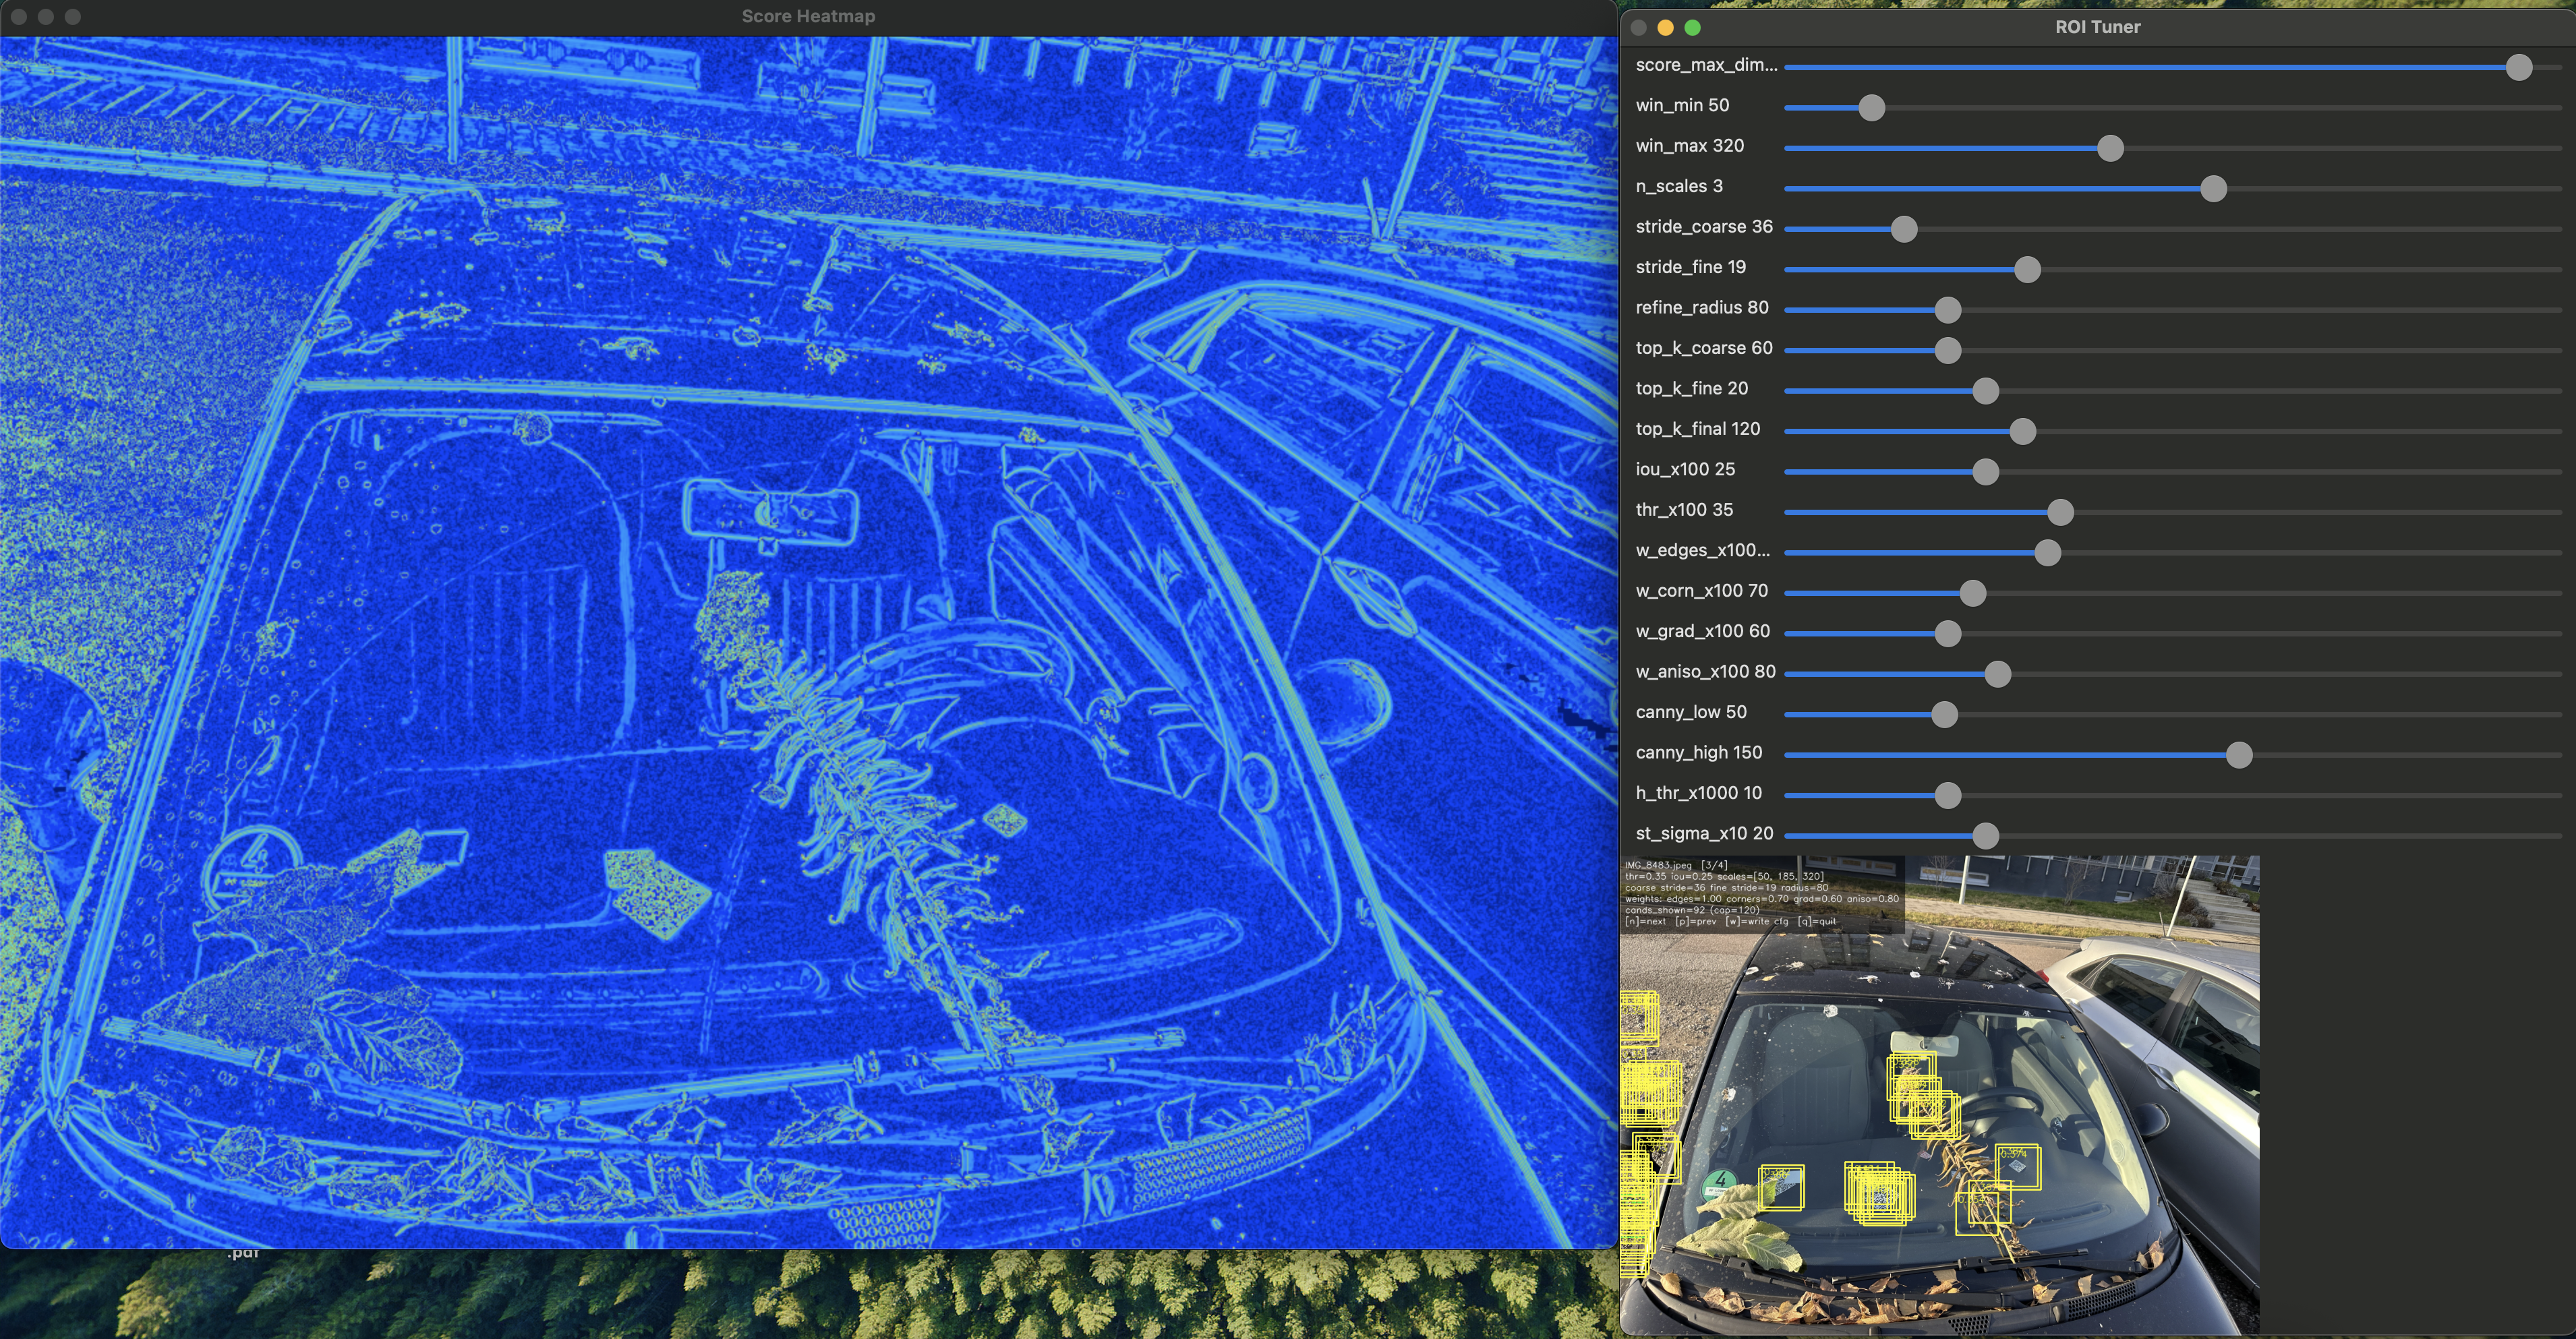
\includegraphics[width=\VarPicWidthD]{Figures/png/roi_tuner_gui.png}
    \caption{ROI-Tuner \ac{GUI}: links Score-Heatmap der kombinierten Merkmale, rechts Parameter-Regler sowie Vorschau der Kandidatenfenster im Originalbild.}
    \label{fig:roi_tuner_gui}
\end{figure}

Zusätzlich wurde ein Click-basiertes Auto-Tuning prototypisch erprobt, um Parameter automatisch zu optimieren. In der Praxis erwies sich dieser Ansatz als nicht ausreichend stabil, da die Optimierung häufig großflächig hohe Score-Werte erzeugte und dadurch die Kandidatenauswahl weniger spezifisch auf \ac{QR}-Codes reagierte. Die finale Parametrisierung wurde daher \ac{GUI}-gestützt manuell vorgenommen.


\section{Data Augmentation}
\label{sec:dataaugmentation}
Um die Robustheit gegenüber realen Variationen (Neigung, Spiegelungen, unterschiedliche Orientierung des Zettels) zu erhöhen, werden einfache geometrische Augmentierungen eingesetzt:

\begin{listNorm}
    \item \textbf{Rotation:} Beim Patch-Export werden optional zusätzlich gedrehte Patch-Varianten erzeugt (zur Abdeckung geneigter \ac{QR}-Codes).
    \item \textbf{Flip:} Positive \emph{QR-Code}-Patches werden horizontal gespiegelt, um die positive Klasse zu erweitern und das Modell gegen Orientierungsvariationen zu stabilisieren.
\end{listNorm}

Die Augmentierungen werden ausschließlich zur robusten \emph{Erkennung} (\emph{QR-Code vorhanden} vs. \emph{nicht vorhanden}) eingesetzt. Die spätere Lesbarkeitsprüfung erfolgt davon getrennt auf den detektierten \ac{QR}-Regionen.

\subsection{Erstellung der Trainings-, Validierungs- und Test-Splits}
\label{subsec:patch_splits}

Nach der Extraktion und manuellen Annotation der \ac{ROI}-Patches (Klassen \texttt{qr} und \texttt{no\_qr}) werden die Daten in Trainings-, Validierungs- und Testdaten aufgeteilt. Die Split-Erstellung erfolgt automatisiert und wird als JSON-Datei gespeichert, sodass keine Daten dupliziert oder in neue Ordnerstrukturen kopiert werden müssen. 

\subsubsection{Leakage-Vermeidung durch gruppierte Splits}
Da aus einem einzelnen Ursprungsbild typischerweise viele, teils stark überlappende Patches entstehen, wäre eine rein zufällige Patch-Aufteilung problematisch: Sehr ähnliche Bildausschnitte desselben Ursprungsbildes könnten in verschiedenen Splits landen und die Evaluierung dadurch künstlich verbessern.  
Um dies zu vermeiden, erfolgt die Aufteilung nicht auf Patch-Ebene, sondern auf \emph{Source}-Ebene. Alle Patches, die aus demselben Ursprungsbild stammen, werden gemeinsam genau einem Split zugeordnet.

\subsubsection{Split-Strategie und Reproduzierbarkeit}
Die Splits werden mit festen Anteilen (Train/Val/Test) erzeugt und über einen festen Zufallsseed (\texttt{seed=42}) deterministisch reproduzierbar gemacht. Die resultierenden Splits umfassen insgesamt 62 eindeutige Sources, verteilt auf 
\begin{listNorm}
    \item Training: 49 Sources,
    \item Validierung: 6 Sources und
    \item Test: 7 Sources
\end{listNorm}

\subsubsection{Balancierung der Klassenverteilung}
Die Rohdaten sind stark unausgeglichen (deutlich mehr \texttt{no\_qr}-Patches als \texttt{qr}-Patches). Für ein stabiles Training des binären Klassifikators wird daher \emph{pro Split} eine 50/50-Verteilung hergestellt. Dazu wird innerhalb jedes Splits die Mehrheitsklasse (\texttt{no\_qr}) zufällig heruntergesampelt, bis die Anzahl der \texttt{no\_qr}-Patches der Anzahl der \texttt{qr}-Patches entspricht (siehe Tabelle~\ref{tab:patch_splits}). 

\subsubsection{Ablageformat (JSON)}
Die fertigen Splits werden als JSON gespeichert. Jede Sample-Instanz enthält den relativen Dateipfad, das Label (\texttt{y=0} für \texttt{no\_qr}, \texttt{y=1} für \texttt{qr}) sowie die zugehörige Source-ID. Dieses Format wird in den Trainingsskripten direkt eingelesen und erlaubt eine saubere, versionierbare Datenaufteilung. 

\begin{table}[htbp]
    \centering
    \caption{Patch-Splits nach Source-gruppierter Aufteilung (keine Source-Überlappung) und 50/50-Balancierung pro Split.}
    \begin{tabular}{lrrrr}
        \hline
        \textbf{Split} & \textbf{Gesamt} & \textbf{no\_qr} & \textbf{qr} & \textbf{Unique Sources} \\
        \hline
        Training     & 4776 & 2388 & 2388 & 49 \\
        Validierung  & 496  & 248  & 248  & 6  \\
        Test         & 864  & 432  & 432  & 7  \\
        \hline
    \end{tabular}
    \label{tab:patch_splits}
\end{table}

